%%%%%%%%%%%%%%%%%%%%%%%%%%%
% PREAMBOLO DEL DOCUMENTO %
%%%%%%%%%%%%%%%%%%%%%%%%%%%
\documentclass[a4paper,11pt,oneside,top=3cm,bottom=3cm,left=3.5cm,right=3.5cm,openright,reqno,table]{book}
\bibliographystyle{ieeetr}


% openany - fa iniziare i capitoli direttamente nella pagina successiva
% openright - fa iniziare i capitoli nella prima pagina destra disponibile 
% fleqn  - allinea le formule a sinistra anzichè centrarle
% leqno - dispone la numerazione delle formule sulla sinistra o destra
% reqno - dispone la numerazione delle formule sulla destra
%
\usepackage{packages}
% Per non appesantire troppo questo file
% quasi tutti i pacchetti usati sono salvati in packages.sty
%
\linespread{1.5}
% Per avere la parola BOZZA scritta su tutte le pagine

% funziona solo in modalità PS
% Invece per i PDF ho risolto così:
% pdftk tesi.pdf background bozza.pdf output tesi_bozza.pdf
%
%%%%%%%%%%%%%%%%%%%%%%%%%%%%%%%%%
%   DOCUMENTO VERO E PROPRIO    %
%%%%%%%%%%%%%%%%%%%%%%%%%%%%%%%%%
\begin{document}
% FRONTESPIZIO %
\begin{titlepage}
\changepage{}{}{}{-7.5 mm}{}{}{}{}{}

\begin{center}

\includegraphics [width=.15\columnwidth, angle=0]{unisa}\\ % height
\vspace{0.5cm}
{\LARGE \scshape Università degli Studi di Salerno}\\
\vspace{0.5cm}
{\Large Dipartimento di Informatica}\\
\vspace{0.1cm}
{\large Corso di Laurea Magistrale in Informatica}\\
\vspace{1.5cm}
{\Large \scshape Corso di Compressione Dati} \\
\vspace{4cm}
{\Huge \bfseries Secure Compression Based on Burrows-Wheeler Transform} \\
\vspace{5cm}

\begin{minipage}[t]{7cm}
\flushleft
\textsc{Studenti} \\
\textbf{Lorenzo Criscuolo} \\
\textbf{Orazio Cesarano} \\
\textbf{Vincenzo Emanuele Martone} \\

\end{minipage}
\hfill
\begin{minipage}[t]{7cm}
\flushright
\textsc{Docente}

Prof. \textbf{Bruno Carpentieri} \\
\end{minipage}

\vspace{1cm}

{\small Anno Accademico 2022-2023}
\end{center}

\end{titlepage}
%

\frontmatter
% quello che segue è in numerazione romana e i capitoli non verranno numerati
% se non si vuole che compaia il numero di pagina basta usare il comando:
%\nonumber

% SOMMARIO %
\cleardoublepage
%\selectlanguage{italian}
\begin{abstract}
Il progetto, svolto nell'ambito del corso di \emph{Compressione Dati}, si pone come obiettivo quello di proporre un'implementazione di un metodo di compressione sicura di testo basato sulla funzione di permutazione nota in letteratura come \emph{Burrows-Wheeler Transform}. Il paper \emph{Secure Compression and Pattern Matching Based on Burrows-Wheeler Transform} \cite{zeng2018secure} tratta tale metodo di compressione, di cui il docente del corso ha fornito un'implementazione preesistente con l'obiettivo di apportare un miglioramento. Tale implementazione propone una versione non ottimizzata dell'algoritmo trattato dal paper di cui sopra causando, in questo modo, un'espansione della dimensione dei dati che vengono forniti in input. Lo scopo dell'implementazione proposta dal presente lavoro è quello di migliorare l'implementazione di cui si dispone. Per raggiungere tale obiettivo verranno effettuate delle modifiche all'implementazione degli algoritmi che compongono la \emph{pipeline}. Tali miglioramenti riguardano sia l'utilizzo del paradigma \emph{multiprocessing} volto alla parallelizzazione dei passi dell'algoritmo, che un adattamento degli algoritmi alla \emph{pipeline} proposta. Verranno, inoltre, effettuate delle revisioni all'implementazione dell'algoritmo \emph{blocky-Move To Front} volte all'individuazione dei valori ottimali dei parametri di cui la versione sicura di tale algoritmo deve tenere conto. Infine verranno svolti dei confronti in termini prestazionali (tempo di esecuzione e rapporto di compressione) tra alcune varianti dell'algoritmo proposto che fanno uso di diversi algoritmi di compressione della famiglia \emph{variable length Prefix Code} al fine di individuare il compressore che meglio si adatta alla strategia proposta ed implementata.  
\\[1cm]
\end{abstract} 

% INDICI %
\phantomsection
\addcontentsline{toc}{chapter}{Indice}
\tableofcontents
% Il simbolo * serve per evitare che comapaia nell'indice
\clearpage
%\listoffigures
%\clearpage
%\listoftables
\cleardoublepage
\phantomsection
\addcontentsline{toc}{chapter}{Elenco delle figure}
% per inserire l'elenco dei simboli e degli acronimi nell'indice
%\printglossary[type=\acronymtype,title=Elenco delle figure]
% Per stampare l'elenco dei simboli
\listoffigures
\cleardoublepage
\phantomsection
\addcontentsline{toc}{chapter}{Elenco delle tabelle}
% per inserire l'elenco dei simboli e degli acronimi nell'indice
%\printglossary[type=\acronymtype,title=Elenco delle figure]
% Per stampare l'elenco dei simboli
\listoftables
\mainmatter
\phantomsection
%\addcontentsline{toc}{chapter}{Introduzione}
\chapter{Introduzione}
\markboth{Introduzione}{}
% [titolo ridotto se non ci dovesse stare] {titolo completo}

\begin{citazione}
Nell'ambito del presente capitolo verrà effettuata una panoramica generale sulle problematiche trattate dal lavoro svolto, motivando la necessità della costruzione di un algoritmo di compressione sicura di testo. Verrà, successivamente, presentata un'idea ad alto livello della soluzione proposta, evidenziando le modalità mediante le quali questa vada a risolvere le problematiche descritte. Infine, verrà descritta la struttura del lavoro presentato in termini di suddivisione in capitoli. 
\end{citazione}
\newpage

\section{Problematiche trattate} { \setstretch{1.3}
Una delle operazioni fondamentali nell'ambito del \emph{processing} delle stringhe è il \textbf{pattern matching}: tale operazione consiste nell'individuazione di tutte le occorrenze di un determinato \emph{pattern} in una data stringa input. È possibile effettuare tale tipo di operazione su dati compressi seguendo diverse strategie, la più semplice delle quali consiste nel decomprimere, in primo luogo, il file per poi successivamente effettuare le operazioni di \emph{pattern matching} sul file decompresso. Per questioni legate alle prestazioni e all'utilizzo della memoria, vengono generalmente preferite strategie che non richiedano una decompressione dei file e che riescano a lavorare sui file compressi. Al fine di raggiungere tale obiettivo è necessario utilizzare indici di dati compressi che, se dovessero essere conservati su server di terze parti, porterebbero a gravi problematiche di privacy e confidenzialità. La soluzione concettualmente più semplice consiste nel cifrare i dati dopo che questi sono stati compressi, seguendo, in questo modo, il paradigma \emph{encryption-after-compression}. Ulteriori approcci studiati in letteratura consistono nell'integrazione di compressione e cifratura in un unico passaggio sfruttando strutture di dati compressi utilizzate nei classici algoritmi di compressione. Diverse ricerche hanno, tuttavia, mostrato che tali approcci presentano diverse problematiche di sicurezza. In particolare il paradigma \emph{encryption-after-compression} risulta essere insicuro anche nell'ambito di noti compressori come \emph{WinZip 9.0} \cite{kohno2004attacking} \cite{phong2010password}, \emph{WinRAR 3.42} \cite{yeo2006security} e \emph{PKZIP 1.10 e 2.04g} \cite{stay2001zip} \cite{biham1994known}. Infine risulta opportuno sottolineare che nessuno degli approcci discussi fino a questo momento risulta essere in grado di conservare le strutture necessarie al pattern matching.
\section{Soluzione proposta} %descrizione della soluzione all'encryption after compression
Le problematiche che sorgono dalla ricerca di una strategia volta alla costruzione di un algoritmo in grado di svolgere le operazioni di \emph{pattern matching} su dati compressi, portano alla necessità di progettare un approccio \emph{ad-hoc} per risolvere i problemi di sicurezza presenti nelle diverse soluzioni discusse. Gli autori del paper \emph{Secure Compression and Pattern Matching Based on Burrows-Wheeler Transform} \cite{zeng2018secure} hanno proposto una soluzione basata su alcuni algoritmi (ben noti in letteratura) revisionati al fine di garantire le proprietà di sicurezza che li rendano adatti ad un utilizzo reale. La \emph{pipeline} proposta dagli autori del paper \cite{zeng2018secure} è costruita come segue:
\begin{itemize}
    \item La stringa input viene data all'algoritmo \textbf{sBWT (scrambled Burrows-Wheeler Transform)}. L'output dell'algoritmo sarà una permutazione della stringa input avente lunghe sequenze di caratteri ripetuti vicini tra loro;
    \item L'output della \emph{sBWT} viene dato in input alla \textbf{bMTF (blocky Move-To-Front}). Sfruttando il fatto che la \emph{sBWT} restituisca lunghe sequenze di caratteri ripetuti vicini tra loro, tale algoritmo costruisce un output contenente lunghe sequenza di \emph{0}; 
    \item L'output della \emph{bMTF} viene dato in input alla \textbf{RLE (Run-Length Encoding)}. Tale algoritmo fornisce una codifica compatta dell'input facendo uso di un contatore per esprimere in maniera concisa le sequenze di \emph{0} ripetuti;
    \item L'ultimo passo della \emph{pipeline} consiste nell'applicazione di un algoritmo di \textbf{Prefix Code} sull'output della \emph{RLE}. La scelta dell'algoritmo di \emph{Prefix Code} influisce sul rapporto di compressione dell'algoritmo complessivo;
\end{itemize}
La pipeline descritta fa uso di un layer di sicurezza implementato dagli algoritmi \emph{sBWT} e \emph{bMTF} che risultano essere, rispettivamente, la revisione degli algoritmi noti in letteratura come \emph{Burrows-Wheeler Transform (BWT)} e \emph{Move-To-Front (MTF)}. L'algoritmo proposto, inoltre, costruisce due strutture dati ausiliarie che vengono sfruttate per il \emph{pattern matching}. Tali strutture vengono opportunamente manipolate al fine di evitare l'introduzione di vulnerabilità che vanno ad intaccare il layer di sicurezza implementato. La costruzione di tali strutture ed il protocollo utilizzato per l'implementazione del pattern matching sono ampiamente trattati in \cite{zeng2018secure}. Il presente lavoro si pone l'obiettivo di effettuare una panoramica dettagliata della pipeline proposta dagli autori del paper \cite{zeng2018secure} e di proporre un'implementazione in \emph{Python} di un algoritmo di compressione \textbf{lossless} sicura di testo che sfrutti tale \emph{pipeline} e che risulti essere quanto più efficiente possibile puntando a massimizzare il fattore di compressione. Risulta, infine, doveroso sottolineare che l'algoritmo proposto risulta essere sicuro secondo la definizione di sicurezza denominata \textbf{IND-CPA sicurezza} opportunamente definita dagli autori del paper \cite{zeng2018secure} stesso, dal quale è possibile reperire ulteriori dettagli sull'algoritmo di \emph{pattern matching} e sulle garanzie di sicurezza in termini matematici e formali.
\section{Struttura della tesina} 
La trattazione del presente lavoro viene suddivisa in cinque capitoli di cui viene fornita, di seguito, una breve descrizione:
\begin{itemize}
    \item Il capitolo 1 introduce le problematiche trattate e la soluzione proposta;
    \item Il capitolo 2 effettua una trattazione degli algoritmi utilizzati dalla \emph{pipeline} proposta analizzando le motivazioni che hanno portato alla scelta di tali algoritmi;
    \item Il capitolo 3 analizza gli algoritmi trattati nel precedente capitolo ponendo particolare enfasi sulle scelte implementative che hanno portato all'ottenimento di determinati risultati in termini prestazionali e di fattore di compressione;
    \item Il capitolo 4 descrive l'attività di testing svolta nell'ambito dell'implementazione proposta, presentando i risultati ottenuti utilizzando il \emph{Dataset} considerato;
    \item Il capitolo 5 conclude la trattazione con diverse considerazioni finali sul lavoro svolto e sugli eventuali sviluppi futuri;
\end{itemize}
}
\chapter{Algoritmi utilizzati} %\label{1cap:spinta_laterale}
% [titolo ridotto se non ci dovesse stare] {titolo completo}
%
\begin{citazione}
Nell'ambito del presente capitolo sarà effettuata una trattazione degli algoritmi utilizzati dalla \emph{pipeline} che si intende implementare. La trattazione in questione è volta all'analisi delle motivazioni che hanno portato alla scelta degli algoritmi stessi. Verranno, in primo luogo, descritti nel dettaglio gli algoritmi di base che sono stati scelti per costruire la \emph{pipeline}; successivamente verranno passate a rassegna le modifiche apportate a tali algoritmi al fine di aggiungere un layer di sicurezza alla \emph{pipeline}. 
\end{citazione}
\newpage

\section{Pipeline iniziale}
Gli autori di \cite{zeng2018secure} hanno proposto una \emph{pipeline} composta da diversi algoritmi, alcuni dei quali opportunamente modificati al fine di aggiungere un layer di sicurezza al processo di compressione. Nelle sezioni successive verrà fornita una descrizione delle versioni di base di tali algoritmi volta all'agevolazione della comprensione del funzionamento dell'algoritmo complessivo. L'algoritmo di compressione \emph{lossless} di partenza prenderà in input un testo $T$ da comprimere e sarà composto da \emph{Burrows-Wheeler Transform, Move-To-Front, Run-Length Encoding e Variable Length Prefix Code}, restituendo un testo compresso $C$. Specularmente, l'algoritmo di decompressione prenderà in input il testo compresso $C$ e sarà composto da \emph{Inverse Variable Length Prefix Code, Inverse Run-Length Encoding, Inverse Move-To-Front e Inverse Burrows-Wheeler Transform}, restituendo il testo non compresso di partenza $T$.
\subsection{Burrows-Wheeler Transform} 
La \textbf{Burrows-Wheeler Transform (BWT)} è un algoritmo utilizzato in diversi programmi di compressione come \emph{bzip}, tuttavia è importante precisare che non si tratta di un algoritmo di compressione in quanto ha come unico scopo quello di permutare l'ordine dei caratteri della stringa input. Il funzionamento della \emph{BWT} si suddivide in tre step fondamentali:
\begin{enumerate}
    \item Data una stringa input $S$ definita su un alfabeto $\Sigma$, si aggiunge un carattere speciale $\$ \notin \Sigma$ alla fine della stringa $S$ ottenendo la stringa $S'$. Il carattere $\$$ sarà più piccolo in ordine lessicografico rispetto ad ogni altro carattere di $\Sigma$;
    \item Si costruisce una matrice $M$ le cui righe sono gli shift ciclici di $S'$;
    \item Si dispongono le righe di $M$ in ordine lessicografico ottenendo la matrice $M'$ e si restituisce l'ultima colonna di $M'$ come risultato della \emph{BWT};
\end{itemize}
I vantaggi dell'utilizzo della \emph{BWT} risiedono in due fattori principali. In primo luogo tale algoritmo tende a permutare i caratteri della stringa input ponendo quelli ripetuti vicini tra loro, grazie al fatto che le righe della matrice vengono disposte in ordine lessicografico. Ciò fa sì che la stringa restituita dalla \emph{BWT} sia facilmente comprimibile ed è proprio questa caratteristica dell'output ad aver influenzato la scelta dei successivi algoritmi utilizzati nella \emph{pipeline}. La caratteristica appena descritta può facilmente essere ottenuta da un semplice algoritmo che effettua un ordinamento lessicografico dei caratteri della stringa di input; la peculiarità di tale trasformata risiede nel fatto che sia reversibile, fungendo, dunque da base solida per un algoritmo di compressione \emph{lossless}. 
L'algoritmo che inverte la trasformata prende in input il risultato $R$ della \emph{BWT} (dunque l'ultima colonna della matrice). Dal momento che tale colonna contiene tutti i caratteri del testo, basterà effettuarne un ordinamento lessicografico per ottenere la prima colonna della matrice originale ordinata. $R$ e la prima colonna, poste vicine tra loro, formano tutte le coppie di caratteri consecutivi dell'input. Si ordinano tali coppie ottenendo la prima e la seconda colonna della matrice originale ordinata. Si itera tale processo affiancando $R$ e le coppie appena costruite e dopo aver effettuato un ordinamento lessicografico delle triple si ottengono le prime tre colonne della matrice originale. Tale processo viene iterato fino ad ottenere la matrice originale. La riga che termina con il carattere $\$$ conterrà l'input della trasformata. \\
\begin{figure}[h]
    \centering
    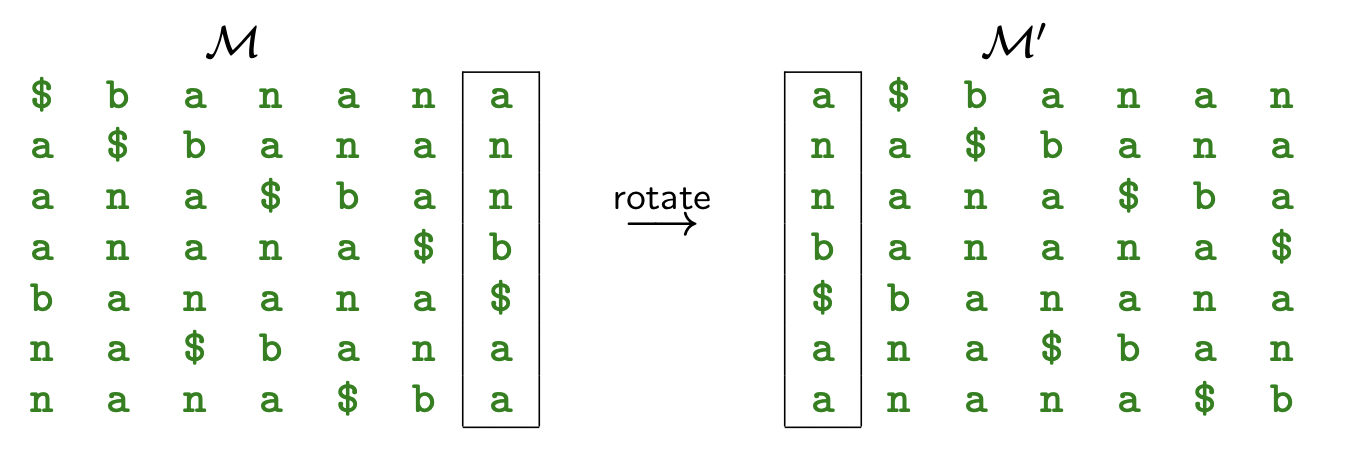
\includegraphics[width=1\textwidth]{Progetto Compressione Dati/capitoli/images/bwt.png}
\caption{Fonte: https://www.cs.helsinki.fi/u/tpkarkka/opetus/12k/dct/lecture08.pdf}
    \label{fig:bwt}
\end{figure}

\begin{figure}[h]
    \centering
    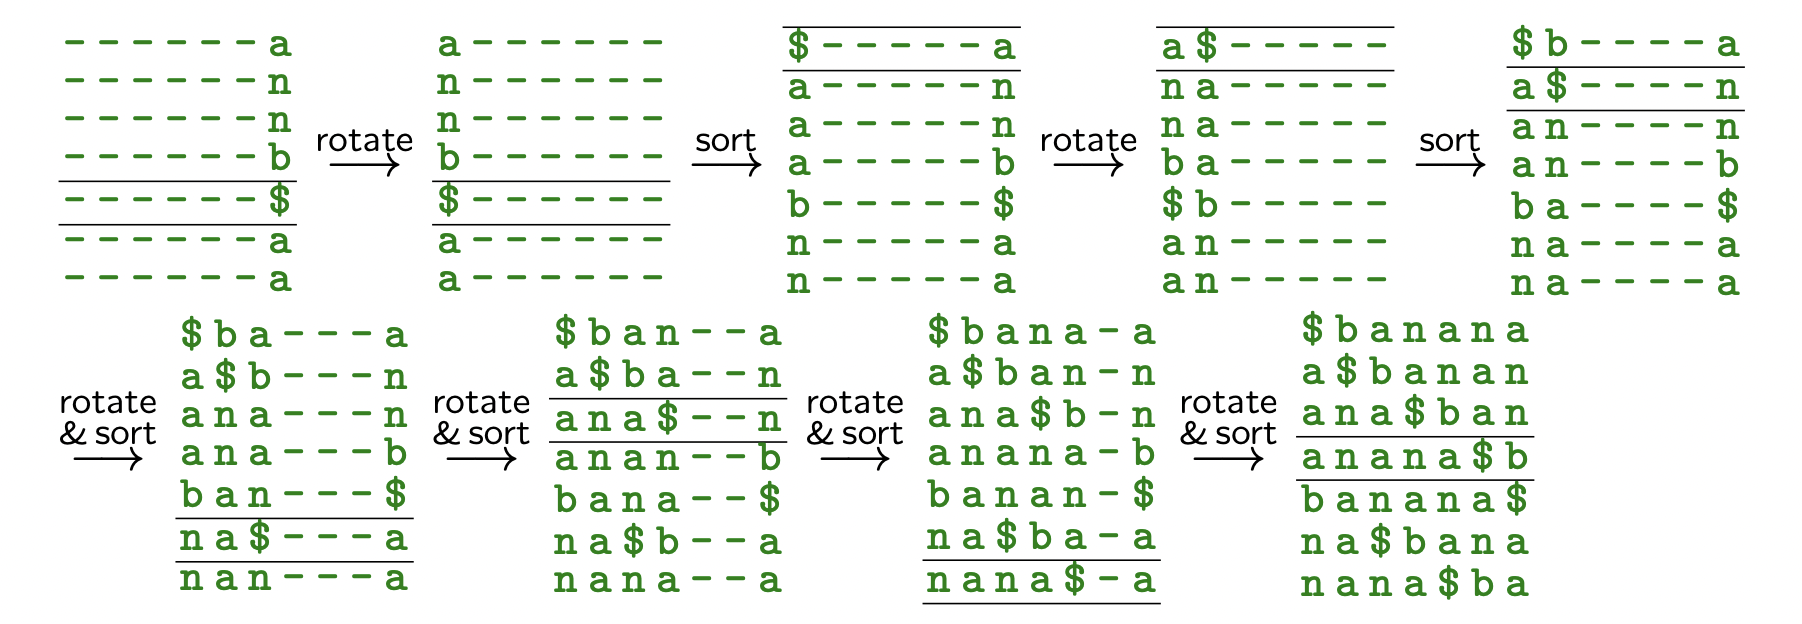
\includegraphics[width=1\textwidth]{Progetto Compressione Dati/capitoli/images/ibwt.png}
\caption{Fonte: https://www.cs.helsinki.fi/u/tpkarkka/opetus/12k/dct/lecture08.pdf}
    \label{fig:ibwt}
\end{figure}

Le figure \ref{fig:bwt} e \ref{fig:ibwt} chiariscono il funzionamento della trasformata e della sua inversa mediante un semplice esempio. 
\subsection{Move-to-Front} \label{section:mtf}
La \textbf{Move-to-Front (MTF)} è un algoritmo di codifica dei dati che consiste nel sostituire ogni simbolo della stringa input con la sua posizione in un alfabeto. Il funzionamento della \emph{MTF} si suddivide in tre step fondamentali:
\begin{enumerate}
    \item Data una stringa input $S$ definita su un alfabeto $\Sigma$, viene costruita una lista $L$ composta dai simboli di $\Sigma$ disposti secondo un certo ordinamento $K$;
    \item Per ogni simbolo $s$ di $S$ si codifica $s$ con la sua posizione $p$ in $L$, si aggiunge $p$ alla stringa $O$ da restituire in output e si sposta $s$ in cima alla lista $L$;
    \item L'output dell'algoritmo sarà la stringa $O$ e l'ordinamento $K$;
\end{enumerate}
Il vantaggio dell'utilizzo della \emph{MTF} risiede nel fatto che nel caso di input aventi lunghe sequenze di caratteri uguali, costruirà output aventi lunghe sequenze di $0$ in quanto i caratteri ripetuti avranno sempre la stessa posizione nell'alfabeto (che sarà proprio 0). La \emph{MTF} risulta essere invertibile a patto di conoscere l'ordinamento $K$ dei simboli dell'alfabeto $\Sigma$. Sostituendo, infatti, ogni simbolo della stringa codificata (che sarà un insieme di posizioni) con il carattere corrispondente nell'alfabeto $\Sigma$ al quale viene applicato l'ordinamento $O$ e portando tale carattere in cima all'alfabeto ad ogni iterazione, è possibile risalire alla stringa input. 
\begin{figure}[h]
    \centering
    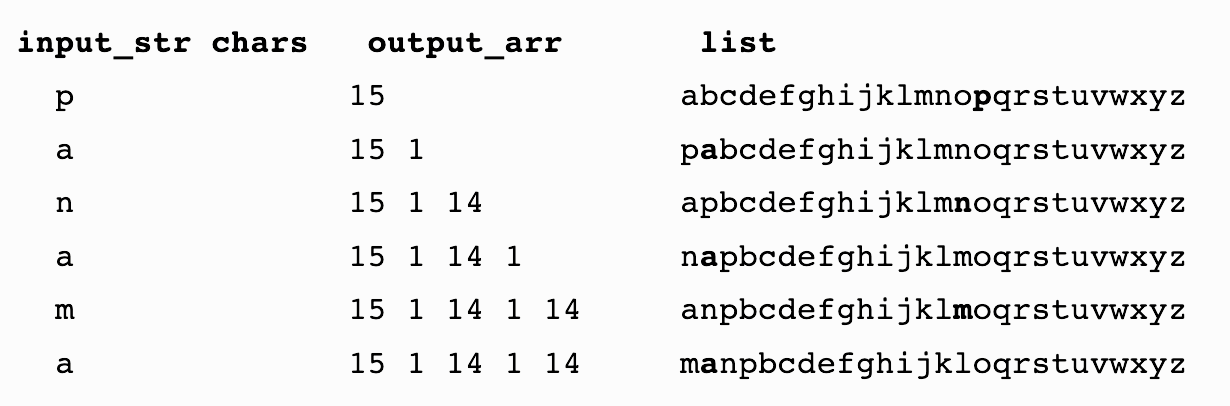
\includegraphics[scale=0.50]{Progetto Compressione Dati/capitoli/images/mtf.png}
\caption{Fonte: https://www.geeksforgeeks.org/move-front-data-transform-algorithm/}
    \label{fig:mtf}
\end{figure}
\begin{figure}[h]
    \centering
    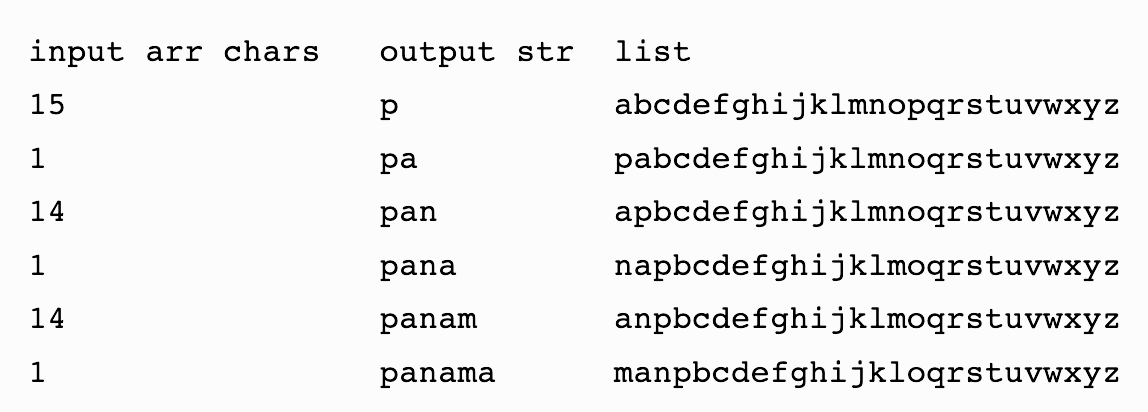
\includegraphics[scale=0.50]{Progetto Compressione Dati/capitoli/images/imtf.png}
\caption{Fonte: https://www.geeksforgeeks.org/inverting-move-front-transform/}
    \label{fig:imtf}
\end{figure} \\
Le figure \ref{fig:mtf} e \ref{fig:imtf} chiariscono il funzionamento della \emph{MTF} e della sua inversa mediante un semplice esempio. 

\subsection{Run-length encoding} \label{section:rle}
La \textbf{Run-length encoding} è il primo algoritmo di compressione che viene effettivamente utilizzato nella \emph{pipeline}. Tale algoritmo consiste nel rappresentare sequenze di caratteri ripetuti di una stringa in maniera compatta mediante l'utilizzo di un contatore, sostituendo le occorrenze multiple del carattere ripetuto in questione con una coppia $(c, counter)$, dove $c$ è il carattere ripetuto stesso e $counter$ indica il numero di volte in cui tale carattere si ripete. Tale algoritmo è banalmente invertibile sostituendo ogni coppia $(c, counter)$ con un numero di occorrenze di $c$ pari a $counter$. Il vantaggio dell'utilizzo della \emph{RLE} risiede nel fatto che, lavorando sull'output delle precedenti trasformate, si troverà a comprimere stringhe aventi lunghe sequenze consecutive di $0$. Tale caratteristica dell'input fa in modo che questo possa essere rappresentata in maniera concisa riducendone significativamente la lunghezza.  
\begin{figure}[h]
    \centering
    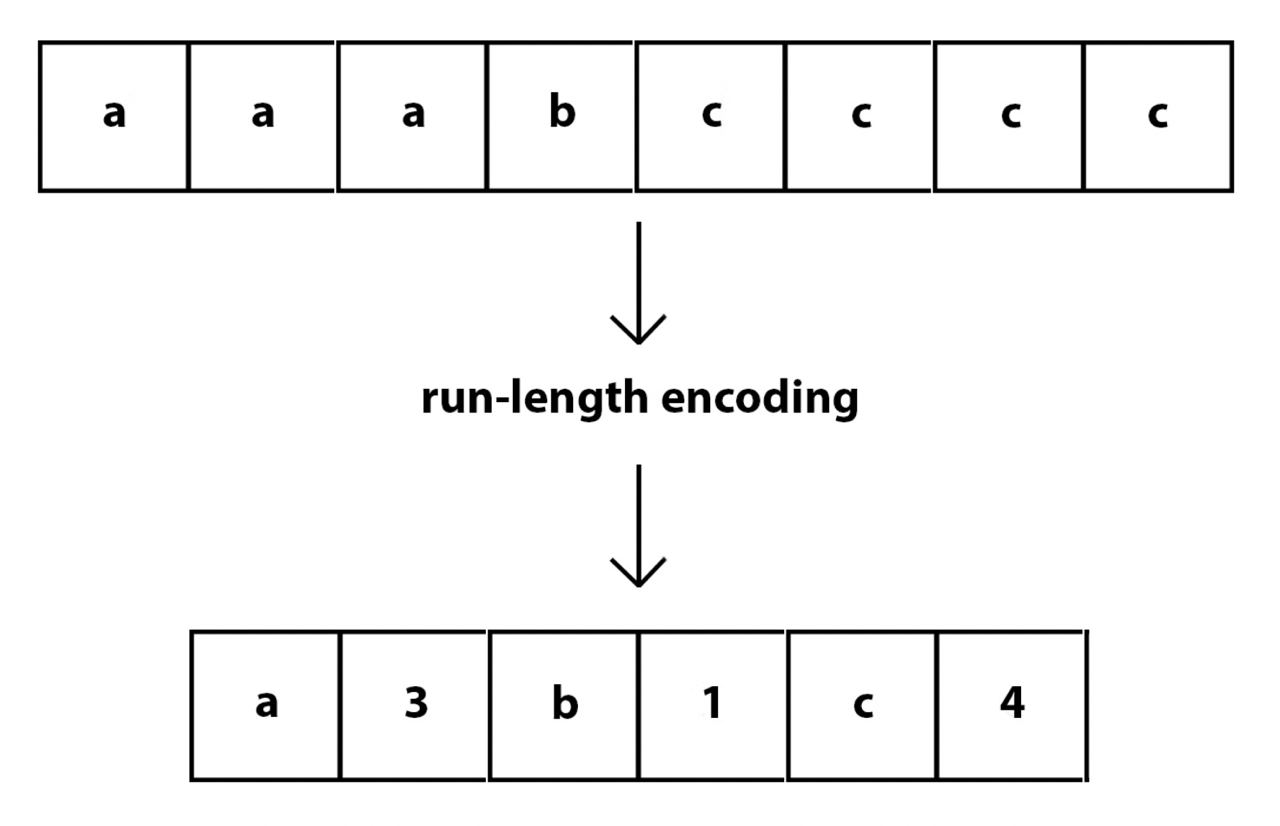
\includegraphics[width=0.5\textwidth, scale=0.5]{Progetto Compressione Dati/capitoli/images/rle.jpg}
\caption{Fonte: https://api.video/what-is/run-length-encoding}
    \label{fig:rle}
\end{figure} \\
La figura \ref{fig:rle} chiarisce il funzionamento della \emph{RLE} mediante un semplice esempio.
\subsection{Variable length Prefix Code} 
In generale, un algoritmo di \textbf{Variable length Prefix Code} consiste nel mappare i simboli della stringa sorgente su un numero variabile di bit. Alcune delle codifiche più note in letteratura sono \emph{Huffman coding}, \emph{Lempel-Ziv-Welch coding} e \emph{Arithmetic coding}. La scelta dell'algoritmo di \emph{Variable length Prefix Code} da inserire nella \emph{pipeline} influisce sul rapporto di compressione dell'algoritmo complessivo. Risulta opportuno sottolineare che tali algoritmi, essendo reversibili, possono essere utilizzati per la costruzione di un algoritmo di compressione \emph{lossless}.  
\section{Pipeline sicura}
La \emph{pipeline} presentata nel paragrafo precedente è strutturata in modo da far lavorare ogni algoritmo che la compone in sinergia con gli altri. Ciascun algoritmo descritto risulta, inoltre, facilmente invertibile, ragion per cui è possibile definire il processo di compressione complessivo \emph{lossless}. Ciò che manca a tale algoritmo è un layer di sicurezza, agevolmente implementabile negli algoritmi descritti mediante opportune modifiche che saranno trattate di seguito. Gli algoritmi interessati da tali modifiche sono la \emph{Burrows-Wheeler Transform} di cui verrà fornita la variante sicura denominata \emph{Scrambled Burrows-Wheeler Transform} e la \emph{Move-to-Front} di cui verrà fornita la versione sicura denominata \emph{Blocky Move-to-Front}. Il motivo per il quale è necessario distribuire il layer di sicurezza su due algoritmi risiede nel fatto che precedenti tentativi da parte di ricercatori di costruire un algoritmo modificando unicamente la \emph{BWT} hanno "scoperto il fianco" ad attacchi di tipo statistico \cite{stanek2012attacking}. Attuando opportune modifiche alla \emph{MTF} è possibile rendere l'algoritmo di compressione complessivo sicuro rispetto a tali attacchi. L'algoritmo di compressione \emph{lossless} sicuro prenderà in input un testo $T$ da comprimere e una chiave segreta $K$ e sarà composto da \emph{Scrambled Burrows-Wheeler Transform, Blocky Move-To-Front, Run-Length Encoding e Variable Length Prefix Code}, restituendo un testo compresso $C$. Specularmente, l'algoritmo di decompressione prenderà in input il testo compresso $C$ e la chiave segreta $K$ e sarà composto da \emph{Inverse Variable Length Prefix Code, Inverse Run-Length Encoding, Inverse Blocky Move-To-Front e Inverse Scrambled Burrows-Wheeler Transform}, restituendo il testo non compresso di partenza $T$. La sicurezza della \emph{pipeline} appena descritta poggia le proprie fondamenta sul concetto di \textbf{IND-CPA sicurezza}. Intuitivamente, tale nozione di sicurezza garantisce che un avversario a cui non è nota la chiave segreta $K$ non sia in grado di stabilire se un testo compresso $C$ sia il risultato della compressione sicura di una stringa $T_0$ o di una stringa $T_1$ (dove $T_0$ e $T_1$ sono stringhe \emph{isomorfe}\footnote{Due stringhe $s$ e $t$ sono isomorfe se ogni occorrenza di ogni carattere di $s$ può essere sostituita per ottenere $t$ mantenendo l'ordinamento dei caratteri, e.g., \emph{egg} e \emph{add} sono stringhe isomorfe, mentre \emph{foo} e \emph{bar} non lo sono.} scelte dall'avversario stesso che ha accesso ad un oracolo di compressione che comprime utilizzando $K$) sfruttando una strategia migliore del "tirare a indovinare". Gli autori di \cite{zeng2018secure} forniscono, oltre che una definizione formale di \emph{IND-CPA sicurezza}, una prova del fatto che l'algoritmo in questione sia \emph{IND-CPA sicuro}. Nei prossimi paragrafi verranno descritte le modifiche da apportare agli algoritmi per far sì che l'algoritmo di compressione soddisfi tale nozione di sicurezza. 
\subsection{Scrambled Burrows-Wheeler Transform} \label{section:sbwt}
Per aggiungere un layer di sicurezza alla \emph{BWT} è possibile modificarla in modo tale che questa prenda in input una chiave segreta $K$, mediante la quale viene calcolato un ordinamento lessicografico segreto che servirà per disporre le righe della matrice generata dall'algoritmo. L'algoritmo risultante da tale modifica, denominato \textbf{Scrambled Burrows-Wheeler Transform} prende in input:
\begin{itemize}
    \item una stringa $S$ da comprimere definita su un alfabeto $\Sigma$;
    \item una chiave segreta $K$;
    \item una funzione di permutazione basata su chiave $Perm$;
\end{itemize}
Il funzionamento dell'algoritmo si suddivide in quattro step fondamentali:
\begin{enumerate}
    \item Si sceglie un numero random $r$ e si computa $Perm(r, K)\rightarrow\xi$, dove $\xi$ denota l'ordinamento lessicografico segreto;
    \item Si aggiunge un carattere speciale $\$ \notin \Sigma$ alla fine della stringa $S$ ottenendo la stringa $S'$. Il carattere $\$$ sarà più piccolo in ordine lessicografico rispetto ad ogni altro carattere di $\Sigma$;
    \item Si costruisce una matrice $M$ le cui righe sono gli shift ciclici di $S'$;
    \item Si dispongono le righe di $M$ nell'ordine lessicografico segreto $\xi$ ottenendo la matrice $M'$ e si restituisce l'ultima colonna di $M'$ come risultato della \emph{sBWT};
\end{enumerate}
L'unica differenza tra le due versioni dell'algoritmo risiede nel fatto che mentre nella \emph{BWT} le righe della matrice $M$ vengono disposte in ordine lessicografico, nella \emph{sBWT} tale ordinamento lessicografico varia in base alla chiave $K$. L'utilizzo di un ordinamento lessicografico fa sì che anche le stringhe di output della \emph{sBWT} presentino lunghe sequenze di caratteri ripetuti, dunque il vantaggio intrinseco della \emph{BWT} viene preservato anche nella sua versione sicura. La proprietà di invertibilità della \emph{sBWT} vale a patto di conoscere l'ordinamento lessicografico segreto utilizzato per disporre le righe della matrice $M$. In altri termini è necessario conoscere la chiave segreta $K$, il numero random $r$ generato in fase di compressione e la funzione di permutazione $Perm$. \\
\subsection{Blocky Move-to-front} {\setstretch{1.3}
La modifica da apportare alla \emph{Move-to-front} al fine di aggiungere un layer di sicurezza non differisce molto da quella che interessa la \emph{BWT}. Anche questa revisione dell'algoritmo, infatti, poggia la proprie fondamenta sulla costruzione di permutazioni segrete dell'alfabeto utilizzato. In particolare, la versione sicura della \emph{MTF}, denominata \textbf{Blocky Move-to-front} prende in input: 
\begin{itemize}
    \item una stringa $S$ da comprimere definita su un alfabeto $\Sigma$;
    \item un parametro intero $L$ che indica la dimensione del blocco;
    \item una chiave segreta $K$;
    \item una funzione di permutazione basata su chiave $Perm$;
    \item un vettore di inizializzazione $IV$;
    \item una funzione hash $f$
\end{itemize}
Il funzionamento dell'algoritmo si suddivide in tre step fondamentali:
\begin{enumerate}
    \item La stringa $S$ viene suddivisa in un certo numero di blocchi, ciascuno dei quali costituito da $L$ caratteri;
    \item Per ogni blocco $block_i$ si costruisce una permutazione $Perm(K, IV$ or $f(block_{i-1})) \rightarrow \xi_i$ dei caratteri nell'alfabeto $\Sigma$. Durante la prima iterazione dell'algoritmo il secondo parametro di $Perm$ è $IV$, mentre durante le iterazioni successive sarà l'hash (calcolato mediante la funzione $f$) del blocco precedente;
    \item Per ogni blocco $block_i$ costruito si eseguono gli step classici della $MTF$ utilizzando l'ordinamento segreto computato;
\end{enumerate}
Nel momento in cui la \emph{bMTF} si trova a lavorare sugli output della \emph{sBWT} produce stringhe contenenti lunghe sequenze di $0$. La lunghezza di tali sequenze dipende dal valore del parametro $L$: più grande sarà questo parametro, più lunga sarà la sequenza. Una trattazione relativa alla scelta del parametro $L$ verrà svolta nei capitoli successivi. Dal momento che la \emph{bMTF} lavora permutando l'alfabeto ogni $L$ caratteri non è possibile per un avversario condurre attacchi di tipo statistico come accadeva nel caso in cui l'unico algoritmo della \emph{pipeline} interessato dalle revisioni di sicurezza era la \emph{BWT}. L'invertibilità della \emph{bMTF} è garantita a patto di conoscere le permutazioni corrispondenti ad ogni blocco dell'input. In altri termini è necessario conoscere la chiave segreta $K$, il vettore di inizializzazione $IV$, la dimensione del blocco $L$, la funzione di permutazione $Perm$ e la funzione hash $f$. 
}
\chapter{Implementazione} %\label{1cap:spinta_laterale}
% [titolo ridotto se non ci dovesse stare] {titolo completo}
%

\begin{citazione}
Nell'ambito del presente capitolo verranno trattate le scelte effettuate per l'implementazione degli algoritmi facenti parte della \emph{pipeline} di compressione. Verrà posta particolare attenzione ai dettagli implementativi della \emph{sBWT} in quanto risulta essere l'algoritmo più pesante in termini di spazio occupato e di tempo impiegato. Verrà, successivamente, fornita una descrizione delle strategie impiegate per l'implementazione della \emph{bMTF} e della \emph{RLE}. Il capitolo si conclude con la descrizione della scelta dell'algoritmo di \emph{Variable Length Prefix Code} da utilizzare. 
\end{citazione}
\newpage

\section{Panoramica sullo sviluppo dell'algoritmo} 
La scelta del linguaggio di programmazione da utilizzare per l'implementazione dell'algoritmo di compressione sicuro è ricaduta su \emph{Python}. Tale scelta è stata guidata dalla ricerca di un linguaggio semplice e flessibile che consentisse di implementare in modo agevole e veloce gli algoritmi descritti soffermandosi sui dettagli rilevanti. Il codice sorgente dell'algoritmo sviluppato è reperibile al seguente link: https://github.com/vincenzo-emanuele/Secure-Compression-based-on-BWT. Come mostrato nella figura \ref{fig:project} il progetto è stato suddiviso in 4 \emph{packages}: \emph{sbwt, bmtf, pc e rle}, ognuno dei quali contiene il codice sorgente del corrispondente algoritmo della \emph{pipeline}. L'implementazione delle \emph{pipeline} di compressione e di decompressione è demandato a due file che fungono da tester dei due processi, denominati \emph{compressione.py} e \emph{decompressione.py}. La \emph{pipeline} complessiva è implementata dal file \emph{tester.py} che orchestra l'esecuzione invocando il modulo di compressione e quello di decompressione. La cartella \emph{TestFiles} contiene i file input utilizzati per testare l'algoritmo con i relativi file output prodotti dal processo di compressione.
\begin{figure}[h]
    \centering
    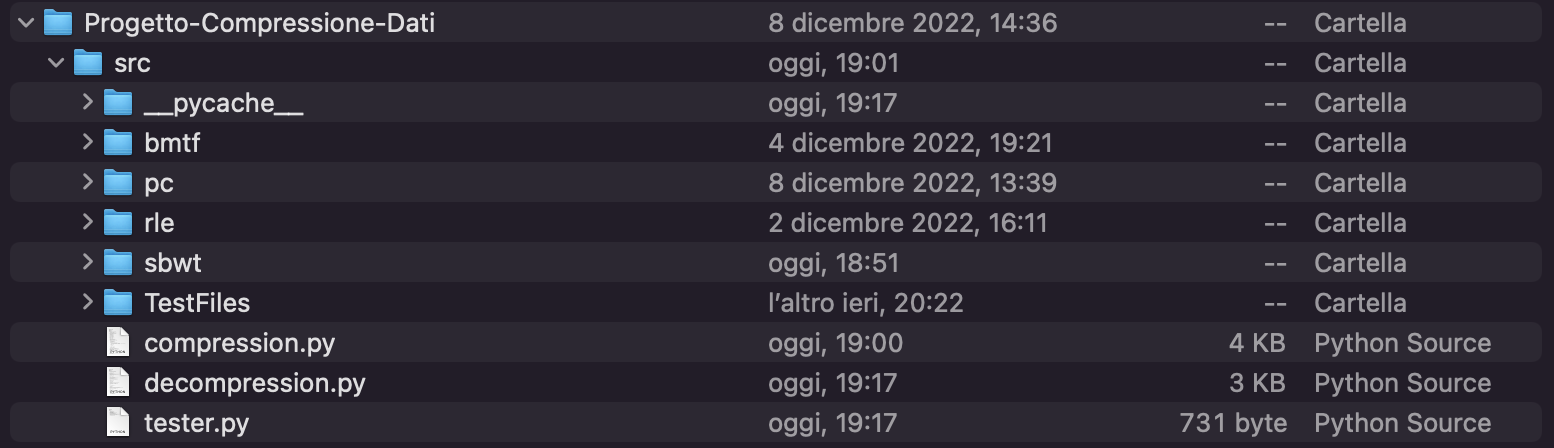
\includegraphics[width=1\textwidth]{Progetto Compressione Dati/capitoli/images/project.png}
\caption{Struttura del progetto}
    \label{fig:project}
\end{figure} \\
\section{Implementazione della sBWT} 
La prima importante questione da affrontare in fase di implementazione della \emph{sBWT} riguarda la realizzazione del layer di sicurezza che si concretizza nell'utilizzo di una chiave segreta per computare un ordinamento lessicografico segreto da utilizzare in fase di disposizione delle righe della matrice.
Risulta, inoltre, necessario affrontare la questione relativa alle prestazioni dell'algoritmo. Implementare la \emph{sBWT} seguendo gli step dell'algoritmo, infatti, non risulta praticabile in quanto la costruzione della matrice porterebbe ad un'esplosione della complessità in termini di tempo e di spazio. Per avere un'idea sulla complessità totale, basti pensare al fatto che la matrice da costruire contiene un numero di elementi pari al quadrato del numero di caratteri della stringa da comprimere; ciò significa che un file di appena 1MB porterebbe alla costruzione di una matrice di 1.099.511.627.776 elementi, occupando oltre 1TB di memoria. Per evitare tali situazioni è possibile applicare diverse ottimizzazioni che poggiano le proprie fondamenta sul fatto di lavorare sulla matrice senza costruirla esplicitamente, facendo uso di strutture ausiliarie costruite \emph{ad-hoc}. I paragrafi successivi descrivono nel dettaglio l'implementazione del layer di sicurezza e le ottimizzazioni attuate.
\subsection{Implementazione del layer di sicurezza}
Nell'ambito del presente lavoro, la realizzazione del layer di sicurezza della \emph{sBWT} è un'implementazione del lavoro svolto dagli autori di \cite{zeng2018secure}. Una descrizione ad alto livello del funzionamento della \emph{sBWT} è stata fornita nel paragrafo \ref{section:sbwt} ed è stata implementata dagli \emph{script} del \emph{package sbwt}. Lo scopo di questo layer di sicurezza è quello di ottenere una permutazione dell'alfabeto su cui è definita la stringa input da comprimere. Nello specifico, mediante la libreria \emph{random} di \emph{Python} viene generato un numero casuale $r$ da 0 a 9999999 che viene salvato su un file denominato \emph{rfile.txt}. A tale $r$ viene accodata la chiave segreta $K$ fornita in input eventualmente dall'utente dell'algoritmo. La chiave risultante $Key=r+K$ viene utilizzata come seed per il generatore di numeri casuali fornito dalla libreria \emph{random} di \emph{Python} mediante il quale vengono generati valori attribuiti a ciascun carattere dell'alfabeto da permutare. In fase di disposizione delle righe della matrice, l'algoritmo di ordinamento farà uso di tale associazione \emph{simbolo dell'alfabeto-numero casuale} creando, così, una permutazione dell'alfabeto input. Tale algoritmo risulta invertibile a patto di salvare il numero casuale $r$ e di conoscere la chiave $K$; infatti, l'utilizzo dello stesso seed $Key=r+K$ fa sì che i numeri casuali ottenuti dal generatore siano esattamente gli stessi, garantendo, in questo modo, l'ottenimento della permutazione dell'alfabeto utilizzata in fase di compressione.
\subsection{Suffix Array}
Al fine di evitare la costruzione esplicita della matrice della \emph{BWT} sono stati utilizzati i \textbf{suffix array}, una struttura dati ben nota nell'ambito degli algoritmi. Formalmente, data una stringa $S$, il \emph{suffix array} $A$ di $S$ è un array di interi contenente le posizioni iniziali dei suffissi di $S$ in ordine lessicografico. Ad esempio, data la stringa $S=banana\$$ (\$ è il carattere speciale di \emph{EOF}), si indicizza la stringa come illustrato nella figura \ref{fig:sa1}.
\begin{figure}[h]
    \centering
    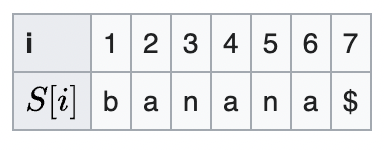
\includegraphics[scale=0.80]{Progetto Compressione Dati/capitoli/images/sa1.png}
\caption{Fonte: https://en.wikipedia.org/wiki/Suffix\_array}
    \label{fig:sa1}
\end{figure}\\
Successivamente si considerano tutti i suffissi: \{\emph{banana\$, anana\$, nana\$, ana\$, na\$, a\$, \$}\} e li si dispone in ordine lessicografico come illustrato nelle figure \ref{fig:sa2} e \ref{fig:sa3}.
\begin{figure}[h]
    \centering
    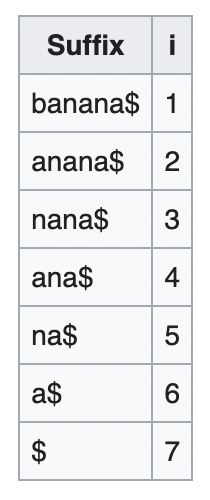
\includegraphics[scale=0.60]{Progetto Compressione Dati/capitoli/images/sa2.png}
\caption{Fonte: https://en.wikipedia.org/wiki/Suffix\_array}
    \label{fig:sa2}
\end{figure}
\begin{figure}[h]
    \centering
    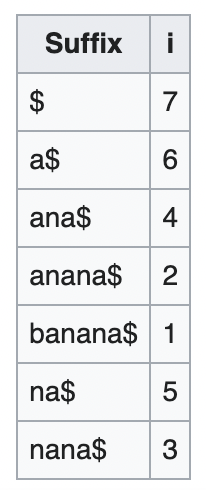
\includegraphics[scale=0.60]{Progetto Compressione Dati/capitoli/images/sa3.png}
\caption{Fonte: https://en.wikipedia.org/wiki/Suffix\_array}
    \label{fig:sa3}
\end{figure}\\
Il \emph{suffix array} risultante sarà $S=\{7, 6, 4, 2, 1, 5, 3\}$. Chiarito il funzionamento della struttura dati in questione, risulta utile descrivere il modo in cui la \emph{sBWT} la utilizza. La matrice $M$ utilizzata dalla \emph{sBWT} contiene, su ogni riga, tutti i suffissi di $S$ ordinati in ordine lessicografico. L'algoritmo computa, in primo luogo, il \emph{suffix array} $A$ relativo a $S$. Dal momento che tale \emph{array} contiene gli indici di tutti i suffissi di $S$ ordinati in ordine lessicografico, vi sarà una corrispondenza biunivoca tra le righe di $M$ e i suffissi "puntati" dagli indici di $A$. In particolare, la \emph{i-esima} riga di $M$ inizierà con il suffisso "puntato" dall'\emph{i-esimo} elemento di $A$. Risulta, dunque, immediato risalire all'ultimo carattere dell'\emph{i-esima} riga di $M$ in quanto sarà proprio l'\emph{i-1-esimo} carattere di $L$. \\ L'ottimizzazione appena descritta riduce la complessità spaziale della \emph{sBWT} da \emph{quadratica} a \emph{lineare}. La complessità temporale, invece, dipende dall'implementazione scelta per la costruzione dei \emph{suffix array}; nell'implementazione proposta dal presente lavoro è stata utilizzata un'implementazione avente complessità $\mathcal{O}(n\log^2{}n)$. Dal momento che la \emph{sBWT}, una volta aver ottenuto il \emph{suffix array}, computa il suo output in tempo $\mathcal{O}(n)$, l'algoritmo complessivo avrà complessità totale $\mathcal{O}(n\log^2{}n)$. La costruzione dei \emph{suffix array} è implementata dalla classe \emph{suffix.py} situata nel package \emph{sbwt}.
\subsection{Variante a blocchi e parallelizzazione}
Al fine di ridurre il tempo richiesto dalla compressione, la \emph{sBWT} viene eseguita su blocchi dell'input di taglia fissata. La dimensione da usare per il blocco è stata scelta in maniera "empirica"; intuitivamente un blocco di dimensione troppo piccola rende meno efficace il raggruppamento dei caratteri effettuato dalla \emph{sBWT} mentre un blocco di dimensione troppo grande rende il \emph{processing} di ciascuno di questi troppo oneroso. Un buon compromesso si ottiene lavorando con blocchi aventi dimensione \emph{300 kB}. Grazie al supporto di \emph{Python} al \emph{multiprocessing} (fornito dalla libreria \emph{multiprocessing}), il \emph{processing} dei blocchi avviene in parallelo, apportando un ulteriore miglioramento al tempo di esecuzione dell'algoritmo.
\subsection{Calcolo dell'inversa} { \setstretch{1.3}
Il calcolo dell'inversa della trasformata è implementato evitando la costruzione esplicita della matrice al fine di scongiurare un'esplosione della complessità. Il paper \cite{burrows1994block} propone una strategia per il calcolo dell'inversa della \emph{BWT} che evita la costruzione della matrice. L'algoritmo prende in input il risultato $L$ della \emph{sBWT}, l'ordinamento lessicografico $O$ utilizzato in fase di compressione e restituisce la stringa non compressa $S$ facendo uso di strutture ausiliarie denominate $C$ e $P$:
\begin{itemize}
    \item $C$ è un dizionario costruito in modo tale che $C[ch]$ è il numero totale di istanze in $L$ dei caratteri che precedono $ch$ nell'ordinamento definito sull'alfabeto;
    \item $P$ è una lista costruita in modo tale che $P[i]$ è il numero di istanze del carattere $L[i]$ nel prefisso $L[0,\dots,i-1]$ di $L$;
\end{itemize}
\begin{figure}[h]
    \centering
    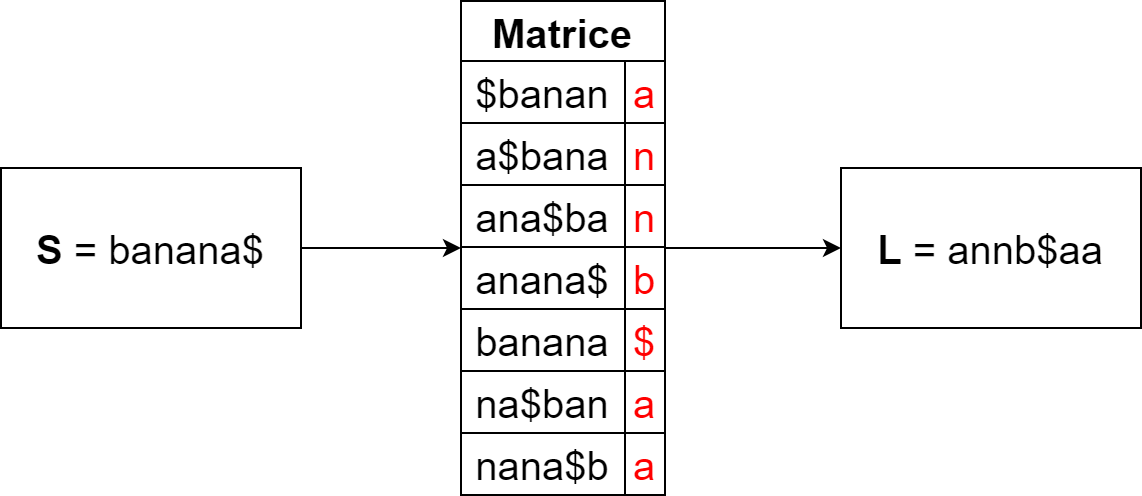
\includegraphics[width=1\textwidth]{Progetto Compressione Dati/capitoli/images/ibwt_ex.png}
\caption{Funzionamento della BWT}
    \label{fig:ibwt_ex}
\end{figure} 
{ \setstretch{1.3}
Grazie a tali strutture, l'algoritmo riesce ad ottenere $S$. Le modalità mediante le quali tale stringa viene costruita si basano sul fatto che non sia necessario costruire esplicitamente una matrice per sfruttarne le proprietà. Dal momento che il funzionamento dell'algoritmo non risulta essere del tutto intuitivo, la sua trattazione verrà affrontata utilizzando come supporto un esempio pratico. Come illustrato nella figura \ref{fig:ibwt_ex} l'output restituito dalla \emph{BWT} sarà l'ultima colonna della matrice ordinata degli shift ciclici di $S$. Dal momento che il carattere di \emph{EOF} è il più piccolo secondo l'ordinamento lessicografico, la prima riga sarà sempre lo shift ciclico che come primo carattere ha l'\emph{EOF} seguito da $S$ (nel caso dell'esempio la riga $0$ della matrice è \emph{\$banana}). Ciò implica che l'ultimo carattere del testo da ricostruire (escludendo l'EOF) è il primo carattere di $L$ ($L[i]$, con $i=0$), in questo caso $a$. Dal momento che per motivi di praticità l'output verrà ricostruito al contrario, il prossimo carattere da individuare è il predecessore di $a$ in $S$. Dato che si dispone solo della stringa $L$, è necessario individuare la riga che termina con il carattere $ch$ cercato in quanto corrisponderà esattamente all'indice di $L$ contenente $ch$; tale riga conterrà i caratteri della riga appena individuata \emph{shiftati} a destra di un carattere, dunque, comincerà con $a$. Sfruttando l'ordinamento della matrice è possibile accedere agevolmente alle righe che cominciano per $a$; a tale scopo risulta utile utilizzare la struttura $C$ in quanto $C[a]$ contiene il numero di occorrenze dei caratteri precedenti ad $a$ nell'ordinamento lessicografico presenti in $L$ (in questo caso $C[a]=1$). La riga $1$ di $M$ inizierà sicuramente per $a$, tuttavia la matrice potrebbe contenere più righe che cominciano con $a$, per cui è necessario stabilire quale di queste contenga come ultimo carattere il predecessore di $a$ cercato. Per fare ciò l'algoritmo si serve della struttura $P$ in quanto $P[i]$ indica quante volte il carattere $L[i]$ (in questo caso $a$) appare all'interno del prefisso $L[0,\dots,i-1]$. Il valore $P[i]$ fungerà da \emph{offset} indicando, tra tutte le righe che cominciano con $a$, quella desiderata. A questo punto, l'algoritmo pone $i=C[L[i]]+P[i]$ e ripete questi passi complessivamente $n$ volte (dove $n$ è la lunghezza di $L$). Ulteriori dettagli sul funzionamento e sulla correttezza di tale algoritmo sono reperibili in \cite{burrows1994block}. 
} }
\section{Implementazione della bMTF}
Il layer di sicurezza implementato nella \emph{bMTF} consiste, in primo luogo, nel suddividere l'input in blocchi di dimensione $L$ per poi, successivamente, eseguire il classico algoritmo di \emph{MTF} descritto nel paragrafo \ref{section:mtf}. Il vantaggio di tale operazione risiede nel fatto che cambiare l'alfabeto periodicamente rende inefficaci attacchi di tipo statistico che poggiano le loro fondamenta sul fatto che uno stesso carattere ripetuto più volte nel testo cifrato corrisponda allo stesso carattere nel testo in chiaro. In altri termini, il cifrario a sostituzione monoalfabetica implementato dalla \emph{sBWT} viene, in questo modo, trasformato in un cifrario a sostituzione polialfabetica rendendo, in questo modo, l'algoritmo aderente alla nozione di \emph{IND-CPA sicurezza}. L'algoritmo in questione è implementato dallo script \emph{bmtf.py} situato nel \emph{package bmtf}. Fa uso di un vettore di inizializzazione noto (per semplicità è \emph{hard-coded}) e di una chiave $K$ fornita eventualmente dall'utente dell'algoritmo, che risulta essere la stessa utilizzata per la \emph{sBWT}. Dopo aver suddiviso l'input in blocchi, ciascuno di dimensione $L$, calcola la permutazione dell'alfabeto da usare per codificare quello specifico blocco facendo uso di un seed $S$ ottenuto dalla concatenazione dell'hash del vettore di inizializzazione (se sta codificando il primo blocco) o dell'hash del blocco precedente (se sta codificando un blocco diverso dal primo) e della chiave $K$. Analogamente a quanto avviene per la \emph{sBWT}, la permutazione dell'alfabeto viene calcolata utilizzando $S$ come seed per il generatore di numeri casuali fornito dalla libreria \emph{random} di \emph{Python}. Un importante questione da trattare nell'ambito dell'implementazione della \emph{bMTF} riguarda la dimensione dei blocchi in cui suddividere l'input. Intuitivamente, blocchi di dimensione troppo grande portano ad un minor numero di permutazioni dell'alfabeto, mentre blocchi di dimensione troppo piccola portano ad una minore efficacia della \emph{bMTF} (in altri termini le sequenze di $0$ saranno più brevi). Il valore da assegnare a $L$ è stato scelto empiricamente ed un buon compromesso è stato raggiunto fissando $L$ a 1024 byte. 
\section{Implementazione della RLE} 
Dal punto di vista implementativo, non sono state apportate modifiche rilevanti alla \emph{RLE} rispetto alla descrizione illustrata nel paragrafo \ref{section:rle}. L'algoritmo è implementato dallo \emph{script rle.py} situato nel \emph{package rle}. 
\section{Scelta dell'algoritmo di PC} 
L'ultimo componente della \emph{pipeline} implementata è l'algoritmo di \emph{variable length Prefix Code}. La scelta dell'algoritmo di \emph{PC} da utilizzare influisce sui tempi di esecuzione e sul rapporto di compressione complessivi. Gli algoritmi di \emph{PC} impiegati nella \emph{pipeline} non sono stati sviluppati da zero ma sono state utilizzate implementazioni in \emph{Python} preesistenti. La scelta dell'algoritmo di \emph{PC} da utilizzare è stata effettuata in maniera empirica in base alle prestazioni riscontrate confrontando tempi di compressione, decompressione e rapporto di compressione; una trattazione approfondita sui risultati ottenuti dal confronto di tali algoritmi è affrontata nel paragrafo \ref{section:risultati}. Lo script \emph{pc.py} situato nel \emph{package pc} implementa gli algoritmi di \emph{PC} utilizzati consentendo, mediante l'utilizzo di un parametro input, di scegliere il compressore desiderato. Nello specifico, gli algoritmi in questione sono: \emph{Huffman Coding}, \emph{Arithmetic Coding}, \emph{Lempel-Ziv-Welch Coding} e \emph{bzip2} (gli ultimi due algoritmi non sono propriamente di \emph{Prefix Code} ma sono stati impiegati al fine di migliorare il rapporto di compressione della \emph{pipeline} proposta).
\section{Implementazione della pipeline}
Nell'ambito dell'implementazione effettuata, gli algoritmi descritti fino a questo momento sono "orchestrati" da un modulo che funge da compressore (reperibile nel \emph{main package src} sotto il nome \emph{compression.py}) e da un modulo che funge da decompressore (reperibile nel \emph{main package src} sotto il nome \emph{decompression.py}). I due moduli vengono, a loro volta, invocati dallo script \emph{tester.py} che si occupa di simulare un \emph{workflow} completo di compressione e decompressione prendendo in input da riga di comando il nome del file da comprimere e la chiave segreta da usare durante la \emph{sBWT} e la \emph{bMTF}. Durante un'esecuzione completa dell'algoritmo di compressione vengono generati diversi file, tuttavia solo una parte di essi va conservata per poter effettuare la decompressione. In particolare i file da conservare sono i seguenti: \emph{outputDictBWT.txt}, \emph{outputPC.txt}, \emph{rfile.txt} e \emph{outputPCCodec.txt} (nel caso in cui viene utilizzato \emph{Huffman}) o \emph{outputDictLZW.txt} (nel caso in cui viene utilizzato \emph{LZW}). D'altro canto, l'algoritmo di decompressione produce un unico file denominato \emph{decompressed.txt} che risulta essere identico al file di input. Dopo l'esecuzione completa della \emph{pipeline}, lo script \emph{tester.py} si occupa di verificare che il file di input sia identico all'output della decompressione.
\chapter{Testing} 

\begin{citazione}
Nell'ambito del presente capitolo verranno descritti i risultati ottenuti dalla fase di testing dell'algoritmo implementato. In primo luogo verrà descritto il \emph{Dataset} impiegato per il testing. Successivamente sarà presentato l'ambiente di esecuzione sul quale è stato eseguito l'algoritmo. In seguito verranno presentati i tempi di esecuzione di compressione e decompressione con i relativi rapporti di compressione effettuando un confronto tra i risultati ottenuti impiegando diversi algoritmi di \emph{variable length Prefix Code}. Infine verrà svolto un paragone tra i risultati ottenuti con la \emph{pipeline} proposta e quelli ottenuti mediante un compressore allo stato dell'arte.
\end{citazione}
\newpage

\section{Dataset}
Dal momento che l'algoritmo implementato lavora solo su testo, il \emph{Dataset} impiegato è costituito da diversi file di testo, di tipologia (racconti, codice sorgente, \dots) e lunghezza variabile. I suddetti file sono reperibili al seguente link: https://github.com/vincenzo-emanuele/Secure-Compression-based-on-BWT/tree/main/src/TestFiles/Input. 
\section{Ambiente di esecuzione}
Per svolgere la fase di testing dell'algoritmo implementato è stato utilizzato un \emph{MacBook Pro M1 (2020)} avente le seguenti specifiche:
\begin{itemize}
    \item S.O.: MacOS Montrey 12.2.1;
    \item CPU: Chip Apple M1;
    \item RAM: 8 GB;
    \item SSD : 512 GB;
    \item Versione di Python installata: 3.8;
\end{itemize}
\section{Risultati}\label{section:risultati}
La fase di testing condotta ha come scopo quello di verificare la bontà dell'algoritmo in termini computazionali (spazio e tempo) e di appurare che la decompressione vada a buon fine senza perdita di informazione, garantendo, dunque, che l'algoritmo di compressione implementato sia \emph{lossless}. Le tabelle \ref{tab:huffman}, \ref{tab:lzw}, \ref{tab:ac} e \ref{tab:bz2pipeline} indicano, per ogni file del \emph{Dataset}, la sua dimensione non compressa, la sua dimensione a seguito della compressione, il tempo impiegato per la compressione (corrisponde al tempo di esecuzione dello script \emph{compression.py} che implementa la \emph{pipeline} di compressione), il tempo impiegato per la decompressione (corrisponde al tempo di esecuzione dello script \emph{decompression.py} che implementa la \emph{pipeline} di decompressione) e il rapporto di compressione ottenuto. In particolare la prima tabella si riferisce alla \emph{pipeline} di compressione che utilizza \emph{Huffman} come algoritmo di \emph{variable length Prefix Code}, la seconda si riferisce alla \emph{pipeline} che fa uso di \emph{Lempel-Ziv-Welch}, la terza si riferisce alla \emph{pipeline} che fa uso di \emph{Arithmetic Coding} mentre la quarta si riferisce alla \emph{pipeline} che utilizza \emph{bzip2} nel suo passo finale.\\ La \emph{pipeline} di testing è implementata dallo script \emph{testing.py} a cui vanno passati i parametri da linea di comando che indicano il nome del file di input e la chiave segreta da utilizzare.\\
Come evidenziato dagli istogrammi \ref{fig:ist1}, \ref{fig:ist2} e \ref{fig:ist3}, non sono state riscontrate differenze evidenti tra l'utilizzo di \emph{Huffman} e quello di \emph{LZW}. Tendenzialmente \emph{Huffman} presenta tempi di esecuzione ed un rapporto di compressione leggermente migliori. Per quanto riguarda \emph{Arithmetic Coding}, è stato rilevato un lieve miglioramento in termini di rapporto di compressione a discapito di un tempo di esecuzione nettamente peggiore. La \emph{pipeline} che indubbiamente si comporta meglio è quella che utilizza \emph{bzip2} raggiungendo un rapporto di compressione più elevato rispetto a quello ottenuto con i precedenti algoritmi.
Dopo aver eseguito le fasi di compressione e decompressione, la \emph{pipeline} di testing si assicura che il processo sia avvenuto in maniera \emph{lossless}. Per fare ciò confronta il file di input con l'output della decompressione: se il contenuto di questi due differisce anche solo di un bit, comunicherà a video il fallimento della decompressione. Tale verifica ha restituito esito positivo su ognuno dei file del \emph{Dataset} utilizzato. Al fine di comprendere la bontà dell'algoritmo implementato è stata svolta un'attività di confronto con lo stato dell'arte della compressione mediante algoritmi basati sulla trasformata di \emph{Burrows-Wheeler}. In particolare il \emph{Dataset} utilizzato per testare l'algoritmo è stato sottoposto al compressore \textbf{bzip2} di cui è stata impiegata un'implementazione \emph{built-in} in \emph{Python} mediante la libreria \emph{bz2}. Dai confronti effettuati (di cui è disponibile un \emph{report} nella tabella \ref{tab:bzip2}) è emerso che \emph{bzip2} nella sua versione \emph{standalone} presenta un fattore di compressione leggermente migliore rispetto a quello della \emph{pipeline} proposta ed un tempo di esecuzione decisamente più basso sia in fase di compressione che in fase di decompressione.
%Huffman
%\begin{center}
    \begin{table}
    \begin{tabular}{||c c c c c c||} 
     \hline
     Input & Size non compr. & Size compr. & Tempo compr. & Tempo decompr. & \% \\ [0.5ex] 
     \hline\hline
     alice29.txt & 152.062 byte & 77.081 byte & 5.44 s & 0.41 s & 49.31\\ [1ex]
     \hline
     asyoulik.txt & 125.179 byte & 68.812 byte & 4.13 s & 0.36 s & 44.14\\ [1ex] 
     \hline
     cp.html & 24.603 byte & 12.342 byte & 0.15 s & 0.03 s & 49.83\\ [1ex] 
     \hline
     fields.c & 11.150 byte & 5.457 byte & 0.16 s & 0.03 s & 51.06\\ [1ex]
     \hline
     grammar.lsp & 3.721 byte & 2.295 byte & 0.04 s & 0.013 s & 38.33\\ [1ex] 
     \hline
     huffman.c & 6.986 byte & 3.582 byte & 0.04 s & 0.008 s & 48.73\\ [1ex]
     \hline
     lcet10.txt & 419.235 byte & 202.267 byte & 9.51 s & 0.70 s & 51.75\\ [1ex] 
     \hline
     manual.ps & 1.766.625 byte & 316.505 byte & 15.69 s & 1.58 s & 82.08\\ 
 [1ex]
     \hline
     plrabn12.txt & 481.861 byte & 265.393 byte & 10.07 s & 0.78 s & 44.92\\ [1ex] 
     \hline
     shrek.txt & 70.658 byte & 40.572 byte & 0.87 s & 0.09 s & 42.58\\ [1ex]

     \hline
    \end{tabular} 
    \caption{Risultati ottenuti con Huffman\label{tab:huffman}}
    \end{table}
%LZW
\begin{table}
    \begin{tabular}{||c c c c c c||} 
     \hline
     Input & Size non compr. & Size compr. & Tempo compr. & Tempo decompr. & \% \\ [0.5ex] 
     \hline\hline
     alice29.txt & 152.062 byte & 81.130 byte & 5.61 s & 0.26 s & 46.65\\ [1ex]
     \hline
     asyoulik.txt & 125.179 byte & 73.462 byte & 4.10 s & 0.22 s & 41.31\\ [1ex] 
     \hline
     cp.html & 24.603 byte & 13.832 byte & 0.40 s & 0.04 s & 43.78\\ [1ex] 
     \hline
     fields.c & 11.150 byte & 5.788 byte & 0.16 s & 0.02 s & 48.09\\ [1ex]
     \hline
     grammar.lsp & 3.721 byte & 2.347 byte & 0.04 s & 0.007 s & 36.93\\ [1ex] 
     \hline
     huffman.c & 6.986 byte & 3.813 byte & 0.09 s & 0.01 s & 45.42\\ [1ex]
     \hline
     lcet10.txt & 419.235 byte & 212.831 byte & 14.40 s & 1.004 s & 49.23\\ [1ex] 
     \hline
     manual.ps & 1.766.625 byte & 330.373 byte & 22.26 s & 2.58 s & 81.30\\ 
 [1ex]
     \hline
     plrabn12.txt & 481.861 byte & 281.687 byte & 15.04 s & 1.14 s & 41.54\\ [1ex] 
     \hline
     shrek.txt & 70.658 byte & 43.728 byte & 2.02 s & 0.13 s & 38.11\\ [1ex]

     \hline
    \end{tabular} 
    \caption{Risultati ottenuti con LZW\label{tab:lzw}}
    \end{table}
%\end{center} 

%Arithmetic Coding
%\begin{center}
    \begin{table}
    \begin{tabular}{||c c c c c c||} 
     \hline
     Input & Size non compr. & Size compr. & Tempo compr. & Tempo decompr. & \% \\ [0.5ex] 
     \hline\hline
     alice29.txt & 152.062 byte & 75.684 byte & 10.3 s & 13.58 s & 50.23\\ [1ex]
     \hline
     asyoulik.txt & 125.179 byte & 68.021 byte & 8.56 s & 12.19 s & 45.66\\ [1ex] 
     \hline
     cp.html & 24.603 byte & 12.792 byte & 0.94 s & 2.14 s & 48.01\\ [1ex] 
     \hline
     fields.c & 11.150 byte & 6.058 byte & 0.51 s & 1.01 s & 45.67\\ [1ex]
     \hline
     grammar.lsp & 3.721 byte & 2.996 byte & 0.21 s & 0.373 s & 19.48\\ [1ex] 
     \hline
     huffman.c & 6.986 byte & 4.217 byte & 0.26 s & 0.578 s & 39.64\\ [1ex]
     \hline
     lcet10.txt & 419.235 byte & 198.395 byte & 22.70 s & 36.29 s & 52.68\\ [1ex] 
     \hline
     manual.ps & 1.766.625 byte & 315.040 byte & 36.06 s & 59.14 s & 82.17\\ 
 [1ex]
     \hline
     plrabn12.txt & 481.861 byte & 260.351 byte & 27.11 s & 46.73 s & 45.97\\ [1ex] 
     \hline
     shrek.txt & 70.658 byte & 40.461 byte & 3.48 s & 7.15 s & 42.74\\ [1ex]

     \hline
    \end{tabular} 
    \caption{Risultati ottenuti con Arithmetic Coding\label{tab:ac}}
    \end{table}

%Bzip2-pipeline
%\begin{center}
    \begin{table}
    \begin{tabular}{||c c c c c c||} 
     \hline
     Input & Size non compr. & Size compr. & Tempo compr. & Tempo decompr. & \% \\ [0.5ex] 
     \hline\hline
     alice29.txt & 152.062 byte & 54.637 byte & 5.48 s & 0.38 s & 64.07\\ [1ex]
     \hline
     asyoulik.txt & 125.179 byte & 49.910 byte & 4.16 s & 0.39 s & 60.13\\ [1ex] 
     \hline
     cp.html & 24.603 byte & 9.568 byte & 0.16 s & 0.03 s & 61.11\\ [1ex] 
     \hline
     fields.c & 11.150 byte & 3.989 byte & 0.17 s & 0.04 s & 64.22\\ [1ex]
     \hline
     grammar.lsp & 3.721 byte & 1.684 byte & 0.05 s & 0.02 s & 54.74\\ [1ex] 
     \hline
     huffman.c & 6.986 byte & 2.721 byte & 0.05 s & 0.018 s & 61.05\\ [1ex]
     \hline
     lcet10.txt & 419.235 byte & 144.068 byte & 9.60 s & 0.78 s & 65.64\\ [1ex] 
     \hline
     manual.ps & 1.766.625 byte & 222.055 byte & 15.71 s & 1.76 s & 87.43\\ 
 [1ex]
     \hline
     plrabn12.txt & 481.861 byte & 188.980 byte & 10.19 s & 0.89 s & 60.79\\ [1ex] 
     \hline
     shrek.txt & 70.658 byte & 29.835 byte & 0.89 s & 0.11 s & 57.78\\ [1ex]

     \hline
    \end{tabular} 
    \caption{Risultati ottenuti con bzip2 nella pipeline\label{tab:bz2pipeline}}
    \end{table}

%BZIP2
\begin{table}
    \begin{tabular}{||c c c c c c||} 
     \hline
     Input & Size non compr. & Size compr. & Tempo compr. & Tempo decompr. & \% \\ [0.5ex] 
     \hline\hline
     alice29.txt & 152.062 byte & 43.172 byte & 0.016 s & 0.005 s & 71.61\\ [1ex]
     \hline
     asyoulik.txt & 125.179 byte & 39.569 byte & 0.013 s & 0.004 s & 68.39\\ [1ex] 
     \hline
     cp.html & 24.603 byte & 7.624 byte & 0.003 s & 0.0007 s & 69.01\\ [1ex] 
     \hline
     fields.c & 11.150 byte & 3.039 byte & 0.002 s & 0.0003 s & 72.74\\ [1ex]
     \hline
     grammar.lsp & 3.721 byte & 1.283 byte & 0.0009 s & 0.0002 s & 65.52\\ [1ex] 
     \hline
     huffman.c & 6.986 byte & 2.110 byte & 0.001 s & 0.0003 s & 69.80\\ [1ex]
     \hline
     lcet10.txt & 419.235 byte & 107.648 byte & 0.03 s & 0.009 s & 74.32\\ [1ex] 
     \hline
     manual.ps & 1.766.625 byte & 162.220 byte & 0.37 s & 0.03 s & 90.82\\ 
 [1ex]
     \hline
     plrabn12.txt & 481.861 byte & 145.545 byte & 0.04 s & 0.01 s & 69.80\\ [1ex] 
     \hline
     shrek.txt & 70.658 byte & 23.346 byte & 0.006 s & 0.003 s & 66.96\\ [1ex]

     \hline
    \end{tabular} 
    \caption{Risultati ottenuti con bzip2\label{tab:bzip2}}
    \end{table}
\begin{figure}[h]
    \centering
    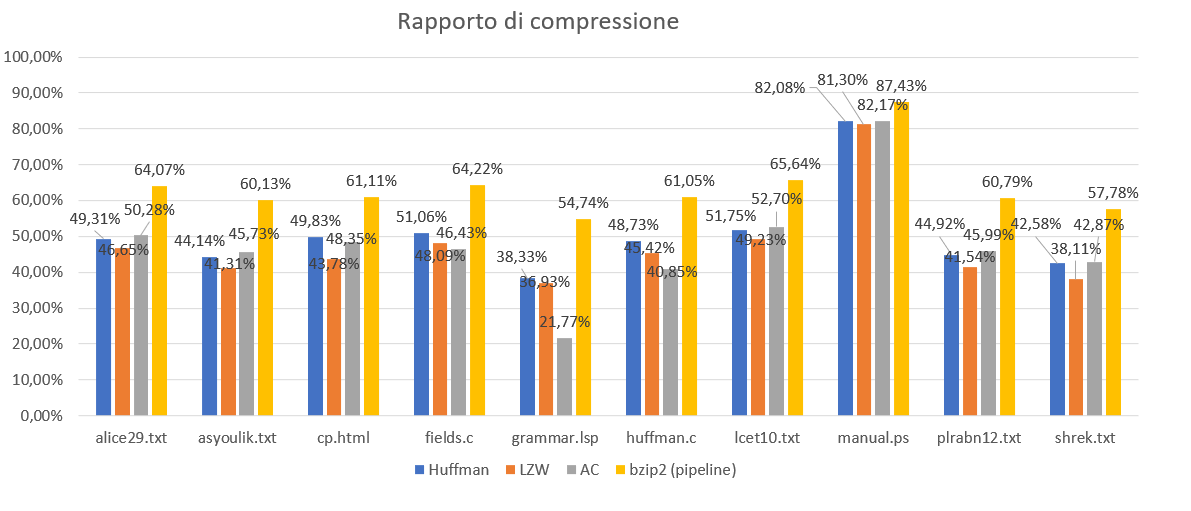
\includegraphics[scale=0.5]{Progetto Compressione Dati/capitoli/images/compression_rate.png}
\caption{Rapporto di compressione}
    \label{fig:ist1}
\end{figure} 
\begin{figure}[h]
    \centering
    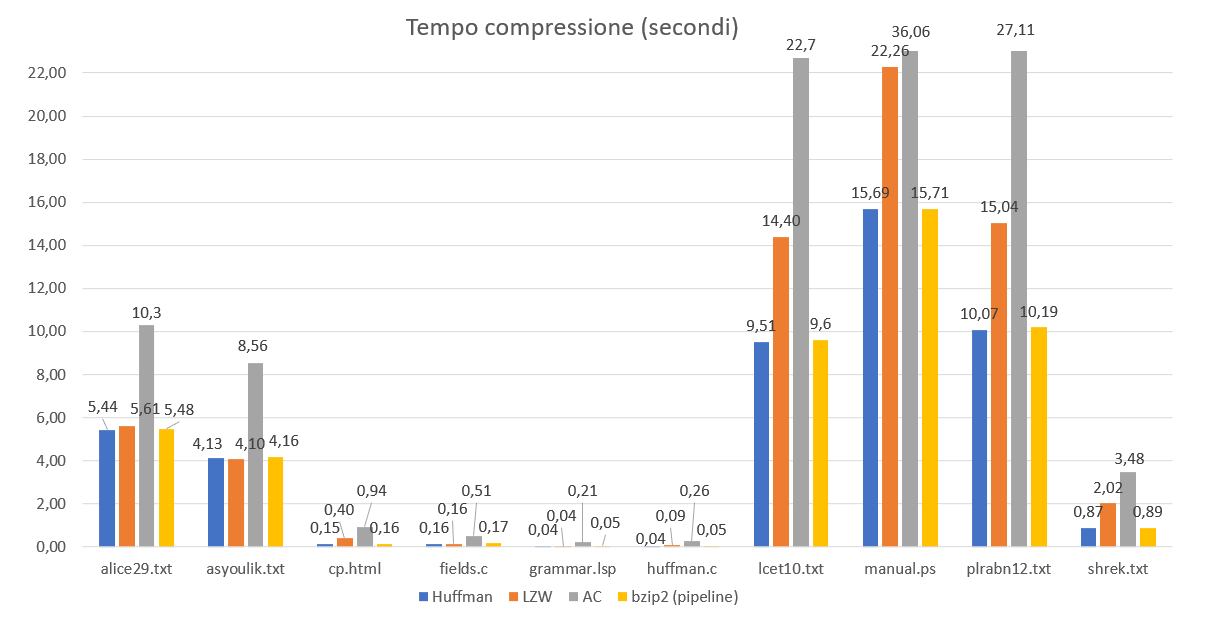
\includegraphics[scale=0.5]{Progetto Compressione Dati/capitoli/images/compression_time.png}
\caption{Tempo di compressione}
    \label{fig:ist2}
\end{figure} 
\begin{figure}[h]
    \centering
    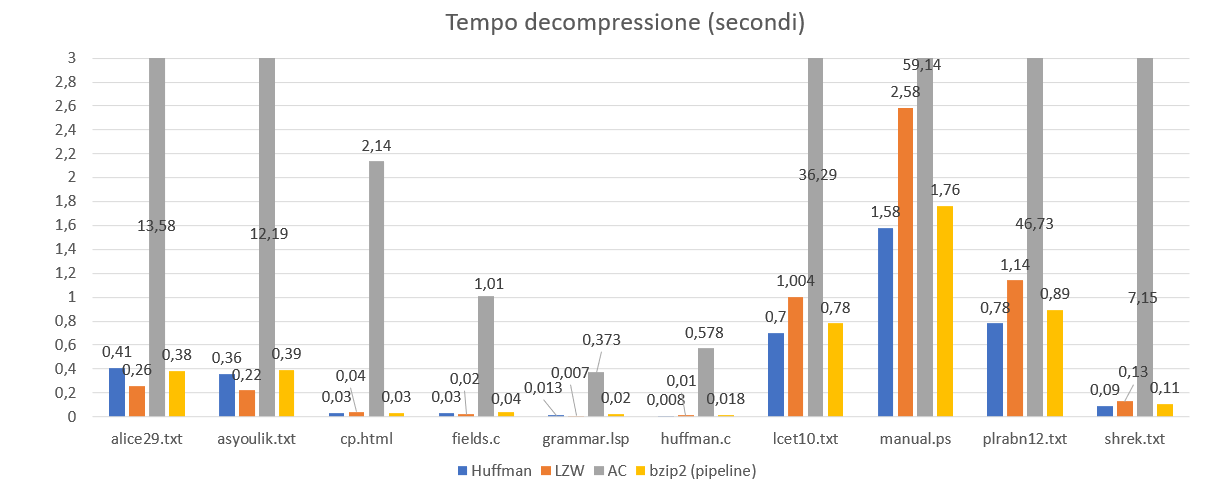
\includegraphics[scale=0.5]{Progetto Compressione Dati/capitoli/images/decompression_time.png}
\caption{Tempo di decompressione}
    \label{fig:ist3}
\end{figure} 
\chapter{Conclusioni} %\label{1cap:spinta_laterale}
% [titolo ridotto se non ci dovesse stare] {titolo completo}
%


\begin{citazione}
Nell'ambito del presente capitolo verranno svolte considerazioni finali sul lavoro effettuato, principalmente dal punto di vista della bontà dell'implementazione proposta. Infine saranno trattati brevemente gli eventuali sviluppi futuri implementabili a partire dal lavoro svolto.
\end{citazione}
\newpage

\section{Considerazioni generali}
La fase di implementazione dell'algoritmo è stata preceduta da uno studio dei diversi componenti della \emph{pipeline} complessiva volto alla comprensione del funzionamento della stessa. Il lavoro svolto si propone come obiettivo quello di essere un'implementazione di \cite{zeng2018secure} e di svolgere un confronto tra alcune varianti dello stesso. Il risultato finale risulta essere un algoritmo di compressione sicuro avente un tasso di compressione che si avvicina al 50\% nel caso del \emph{Dataset} considerato. Inoltre, grazie al layer di sicurezza distribuito su due componenti differenti, l'algoritmo implementato resiste ad attacchi di tipo statistico e risulta essere una solida base per la costruzione di un algoritmo di \emph{pattern matching} che fa uso di indici di dati compressi salvati su \emph{Cloud}.
\section{Sviluppi futuri} % parallelizzazione della IbMTF, ottimizzazione dell'array dei suffissi, implementazione dell'algoritmo di pattern matching
L'algoritmo implementato presenta diversi spunti a partire dai quali è possibile costruire lavori futuri. Nello specifico, risulta possibile:
\begin{itemize}
    \item Apportare miglioramenti all'algoritmo grazie alla parallelizzazione della \emph{I-bMTF} in quanto l'inversione lavora su blocchi tra loro indipendenti utilizzando informazioni note all'inizio della decompressione;
    \item Utilizzare un'implementazione della costruzione dei \emph{suffix array} avente complessità $\mathcal{O}(n)$ al fine di velocizzare la fase di compressione;
    \item Implementare un algoritmo di \emph{pattern matching} che fa uso dell'algoritmo di compressione implementato mediante la costruzione di opportune strutture di supporto;
\end{itemize} 
%*******************************************************
% Bibliografia
%*******************************************************
\cleardoublepage
\phantomsection
\addcontentsline{toc}{chapter}{\bibname}
\nocite{*}
\bibliographystyle{unsrt}
{ \setstretch{1.3}
\bibliography{bibliografia}
}
\vspace{0.5cm}
% \begin{Large}Fonti\end{Large}
% \begin{itemize}
% \end{itemize}


\end{document}
